% !TEX root = ../main.tex
\paragraph{Forward Time-of-Flight (FTOF)}
    \begin{wrapfigure}{r}{0.50\textwidth}
        \frame{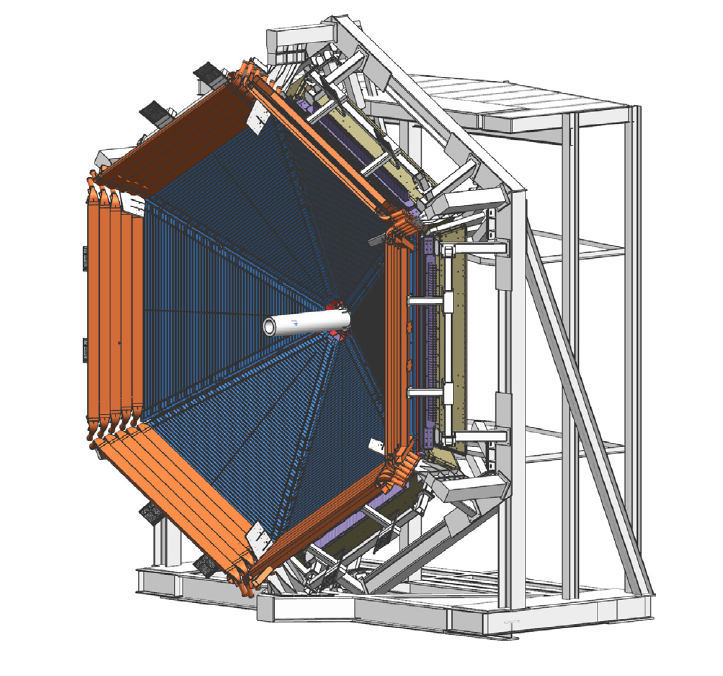
\includegraphics[width=\linewidth]{214ftof.png}}
        \caption[Forward Time-of-Flight (FTOF) system]
        {Render of the Forward Carriage with the FTOF system showing the panel-1b counters on the inside (dark blue), and the panel-2 counters on the outside (bronze).
        The panel-1a counters are located immediately downstream of the panel-1b counters and are not visible in the render.
        Part of the Pre-shower Calorimeter (PCAL) is visible downstream of the FTOF panels.}
        \floatfoot{Source: \href{https://jlab.org/physics/hall-b/clas12}{CLAS12 wiki}.}
        \label{fig::11.214::ftof}
    \end{wrapfigure}

    The FTOF system is designed to measure the time-of-flight of charged particles emerging from the target during beam operation.
    It consists of six sectors of plastic scintillators with double-sided PMT readout.
    Each sector is divided into three arrays of counters separated into panels.
    Panel-1a has 23 counters, panel-1b has 62 counters, and panel-2 has 5 counters.
    The FTOF system is designed to provide excellent timing resolution for particle identification and good segmentation for flexible triggering options.
    The detectors cover a polar angle range from $5\degree$ to $45\degree$, spanning $50\%$ in azimuth at $5\degree$ and $90\%$ at $45\degree$.
    The lengths of the counters vary across the panels, ranging from $32.3 ~\text{cm}$ to $376.1 ~\text{cm}$ in panel-1a, from $17.3 ~\text{cm}$ to $407.9 ~\text{cm}$ in panel-1b, and from $371.3 ~\text{cm}$ to $426.2 ~\text{cm}$ in panel-2.

    The timing resolution achieved in the FTOF system is $125 ~\text{ps}$ in panel-1a, $85 ~\text{ps}$ in panel-1b, and $155 ~\text{ps}$ in panel-2.
    This timing resolution allows for precise measurements of the particle's time-of-flight, which is crucial for particle identification purposes \cite{carman2020ftof}.
    A render of the FTOF detector can be seen in Figure \ref{fig::11.214::ftof}.
